% Prepared by Calvin Kent
%
% Assignment Template v19.02
%
%%% 20xx0x/MATHxxx/Crowdmark/Ax
%
\documentclass[12pt]{article} %
\usepackage{CKpreamble}
\usepackage{CKassignment}
\usepackage{tkz-euclide}
\usepackage{physunits}
\usepackage{physics}
\usepackage{lmodern}
\usepackage{microtype}
\usepackage{upgreek}
\usepackage[misc]{ifsym}

%%% Maths and science packages

\usepackage{amsmath,amsthm,amssymb}
\usepackage{pgfplots}
	\usetikzlibrary{
		calc,
		patterns,
		positioning
	}
	\pgfplotsset{
		compat=1.16,
		samples=200,
		clip=false,
		my axis style/.style={
			axis x line=middle,
			axis y line=middle,
			legend pos=outer north east,
			axis line style={
				->,
			},
			legend style={
				font=\footnotesize
			},
			label style={
				font=\footnotesize
			},
			tick label style={
				font=\footnotesize
			},
			xlabel style={
				at={
					(ticklabel* cs:1)
				},
				anchor=west,
				font=\footnotesize,
			},
			ylabel style={
				at={
					(ticklabel* cs:1)
				},
				anchor=west,
				font=\footnotesize,
			},
			xlabel= $t$,
			ylabel=$\vec d (\m \tx{[East]})$
		},
	}
	\tikzset{
		>=stealth
	}

%%% Tables and figures packages

\usepackage{float}
\usepackage{caption}
	\captionsetup{
		format=plain,
		labelfont=bf,
		font=small,
		justification=centering
	}
	
%%% Numbers and sets

\newcommand{\E}{\mathrm{e}}

\newcommand{\tx}[1]{\text{#1}}

\begin{document}
    \pagenumbering{arabic}
    % Start of class settings ...
    \renewcommand*{\coursecode}{Physics REVIEW} % renew course code
    \renewcommand*{\assgnnumber}{1} % renew assignment number
    \renewcommand*{\submdate}{August 26, 2021} % renew the date
    \renewcommand*{\studentfname}{Abdullah} % Student first name
    \renewcommand*{\studentlname}{Zubair} % Student last name
    %\renewcommand*{\studentnum}{SNumber} % Student number

    \renewcommand\qedsymbol{$\blacksquare$}
    \setfigpath
    % End of class settings 
    \pagestyle{crowdmark}
    \newgeometry{left=18mm, right=18mm, top=22mm, bottom=22mm} % page is set to default values
    \fancyhfoffset[L,O]{0pt} % header orientation fixed
    % End of class settings
    %%% Note to user:
    % CTRL + F <CHANGE ME:> (without the angular brackets) in CKpreamble to specify graphics paths accordingly.
    % The command \circled[]{} accepts one optional and one mandatory argument.
    % Optional argument is for the size of the circle and mandatory argument is for its contents.
    % \circled{A} produces circled A, with size drawn for letter A. \circled[TT]{A} produces circled A with size drawn for TT.
    % https://github.com/CalvinKent/My-LaTeX
    %%%
    % Crowdmark assignment start
\begin{qstn}[1]
Answer the followiing True / False questions \textbf{(Assume [North],[East] is positive)}
\begin{enumerate}
\item I throw a rock $d = 100 \m$ in the air and it returns to my hand in $\Delta t = 20 \s$
	\begin{enumerate}[label = (\alph*)]
		\item The average speed of the ball was $v_{av} = 5 \m / \s$. (T / F)
		\item The average velocity of the ball over $\Delta t = 20 \s$ was $\vec v_{av} = +5 \m / \s$[North]. (T / F)
	\end{enumerate}
\item Suppose a rubber bullet travels at an average speed of $v_{av} = 600 \km / \s$ and an average velocity of $v_{av} = +600 \km / \s$.
	\begin{enumerate}[label = (\alph*)]
		\item The distance it can cover in $\Delta t = 4 \s$ is $d = 2.4 \times 10^6 \m$. (T / F)
		\item Suppose the reference point is $(0,0)$. If the gun is placed at $\vec d_i = +20\m$ and then fired, then after $\Delta t = 2\s$, $\vec d_f = +1.2 \times 10^3\m$. (T / F)
	\end{enumerate}
\item Suppose that the equation of motion for a rocket was $x = -4t - 6$. Then,
	\begin{enumerate}[label = (\alph*)]
		\item The rocket experienced uniform motion. (T / F)
		\item The rocket experienced an average velocity of $\vec v_{av} = -10 \m / \s$. (T / F)
		\item The rocket was initially [West] relative to the reference point. (T / F)
	\end{enumerate}
\item Suppose that a frisbee has an average speed of $v_{av}$ and that it takes $\Delta t$ seconds to reach the end of the room. 
	\begin{enumerate}[label = (\alph*)]
		\item Doubling the average speed of the frisbee will triple the distance it can travel. (T / F)
		\item If I want the frisbee to reach the end of the room in $\frac{\Delta t}{3}$ seconds then I must triple the average speed. (T / F)
	\end{enumerate}
\item Consider the Position V. Time graph for a body in motion below
\begin{figure}[h]
	\centering
	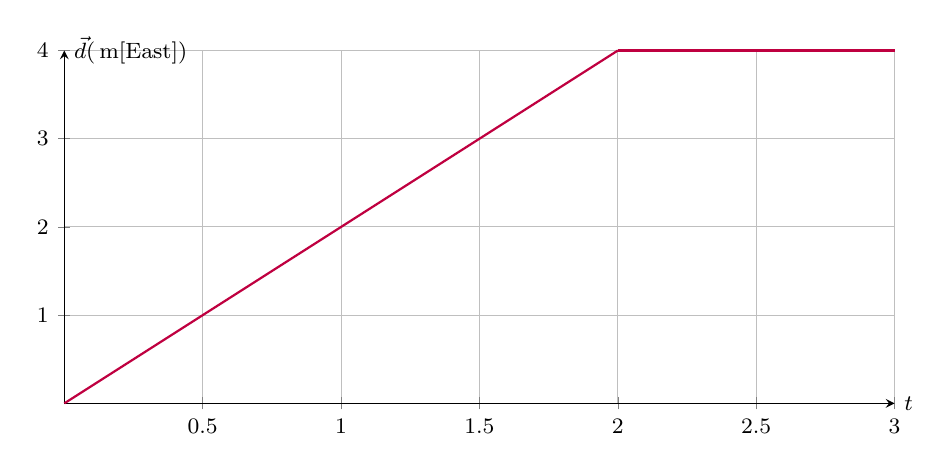
\begin{tikzpicture}
	\begin{axis}[
		my axis style,
		width=\textwidth,
		height=.5\textwidth,
		grid
	]
	
	\addplot[
		domain=0:2,
		thick,
		purple,
		-
	]
	{2*x};

	\addplot[
		domain=2:3,
		thick,
		purple,
		-
	]
	{4};
	
	\fill[
		black
	];
	
	\end{axis}
	\end{tikzpicture}
\end{figure}
	\begin{enumerate}[label = (\alph*)]
		\item The body had an average velocity of $\vec v_{av} = +2 \m / \s$. (T / F)
		\item The body continued to move in the positive direction after $t = 2\s$. (T / F)
	\end{enumerate}

\item On an island there are three points $A,B,C$ that lie on a straight line. There is no information of $\vec d_{AB}$, I would like to obtain this vector. I can obtain this vector if there exists information of,
	\begin{enumerate}[label = (\alph*)]
		\item $\vec d_{AC}$, $\vec d_{BC}$. (T / F)
		\item $\vec d_{CA}$, $\vec d_{CB}$. (T / F)
		\item $\vec d_{AC}$, $\vec d_{CB}$. (T / F)
		\item $\vec d_{BC}$, $\vec d_{CA}$. (T / F)
		\item The average speed and the time elapsed from $A$, $B$. (T / F) 
	\end{enumerate}
 


\end{enumerate}


\end{qstn}



\begin{qstn}[2] % qnumber, qname, qpoints
	Convert the following quantities to $\m / \s$
	\begin{enumerate}[label = (\alph*)]
		\item $120 \mi / \h$
		\vspace*{4cm}

		\item $400 \km / \h$
		\vspace*{4cm}
		
		\item $368 \m / \min$
		\vspace*{4cm}

		\item $678 \inch / \min$
		\vspace*{4cm}

	\end{enumerate}

\end{qstn}


\begin{qstn}[3]
	Compute the \textbf{displacement} (or \emph{net} displacement) given the position vectors. Assume that the reference point is $(0,0)$ for \emph{all} vectors.
    \begin{enumerate}[label=(\alph*)]
        \item $\vec d_1 = 623 \tx{\m}[\tx{East}]$, $\vec d_2 = 412 \tx{\m}[\tx{East}]$
         \vspace*{4cm}
        \item $\vec d_1 = +500\km$, $\vec d_2 = -801\km$, $\vec d_3 = -120\km$, $\vec d_4 = +61\km$, $\vec d_5 = +400\km$, $\vec d_6 = -742\km$.
        \vspace*{12cm}
        \item $\vec d_i = 601\tx{\m}[\tx{Left}]$, $\vec d_f = 234\tx{\m}[\tx{Right}]$
    \end{enumerate}

\end{qstn}

\end{document}



















